\section{Atividade 5 -- Google Dorks}

\paragraph{}
Foram realizados testes utilizando Google Dorks para identificar possíveis
informações sensíveis expostas publicamente.

\subsection{Google Dork Utilizado}

\begin{verbatim}
intitle:"Remote Desktop Web Client"
\end{verbatim}

\begin{figure}[H]
    \centering
    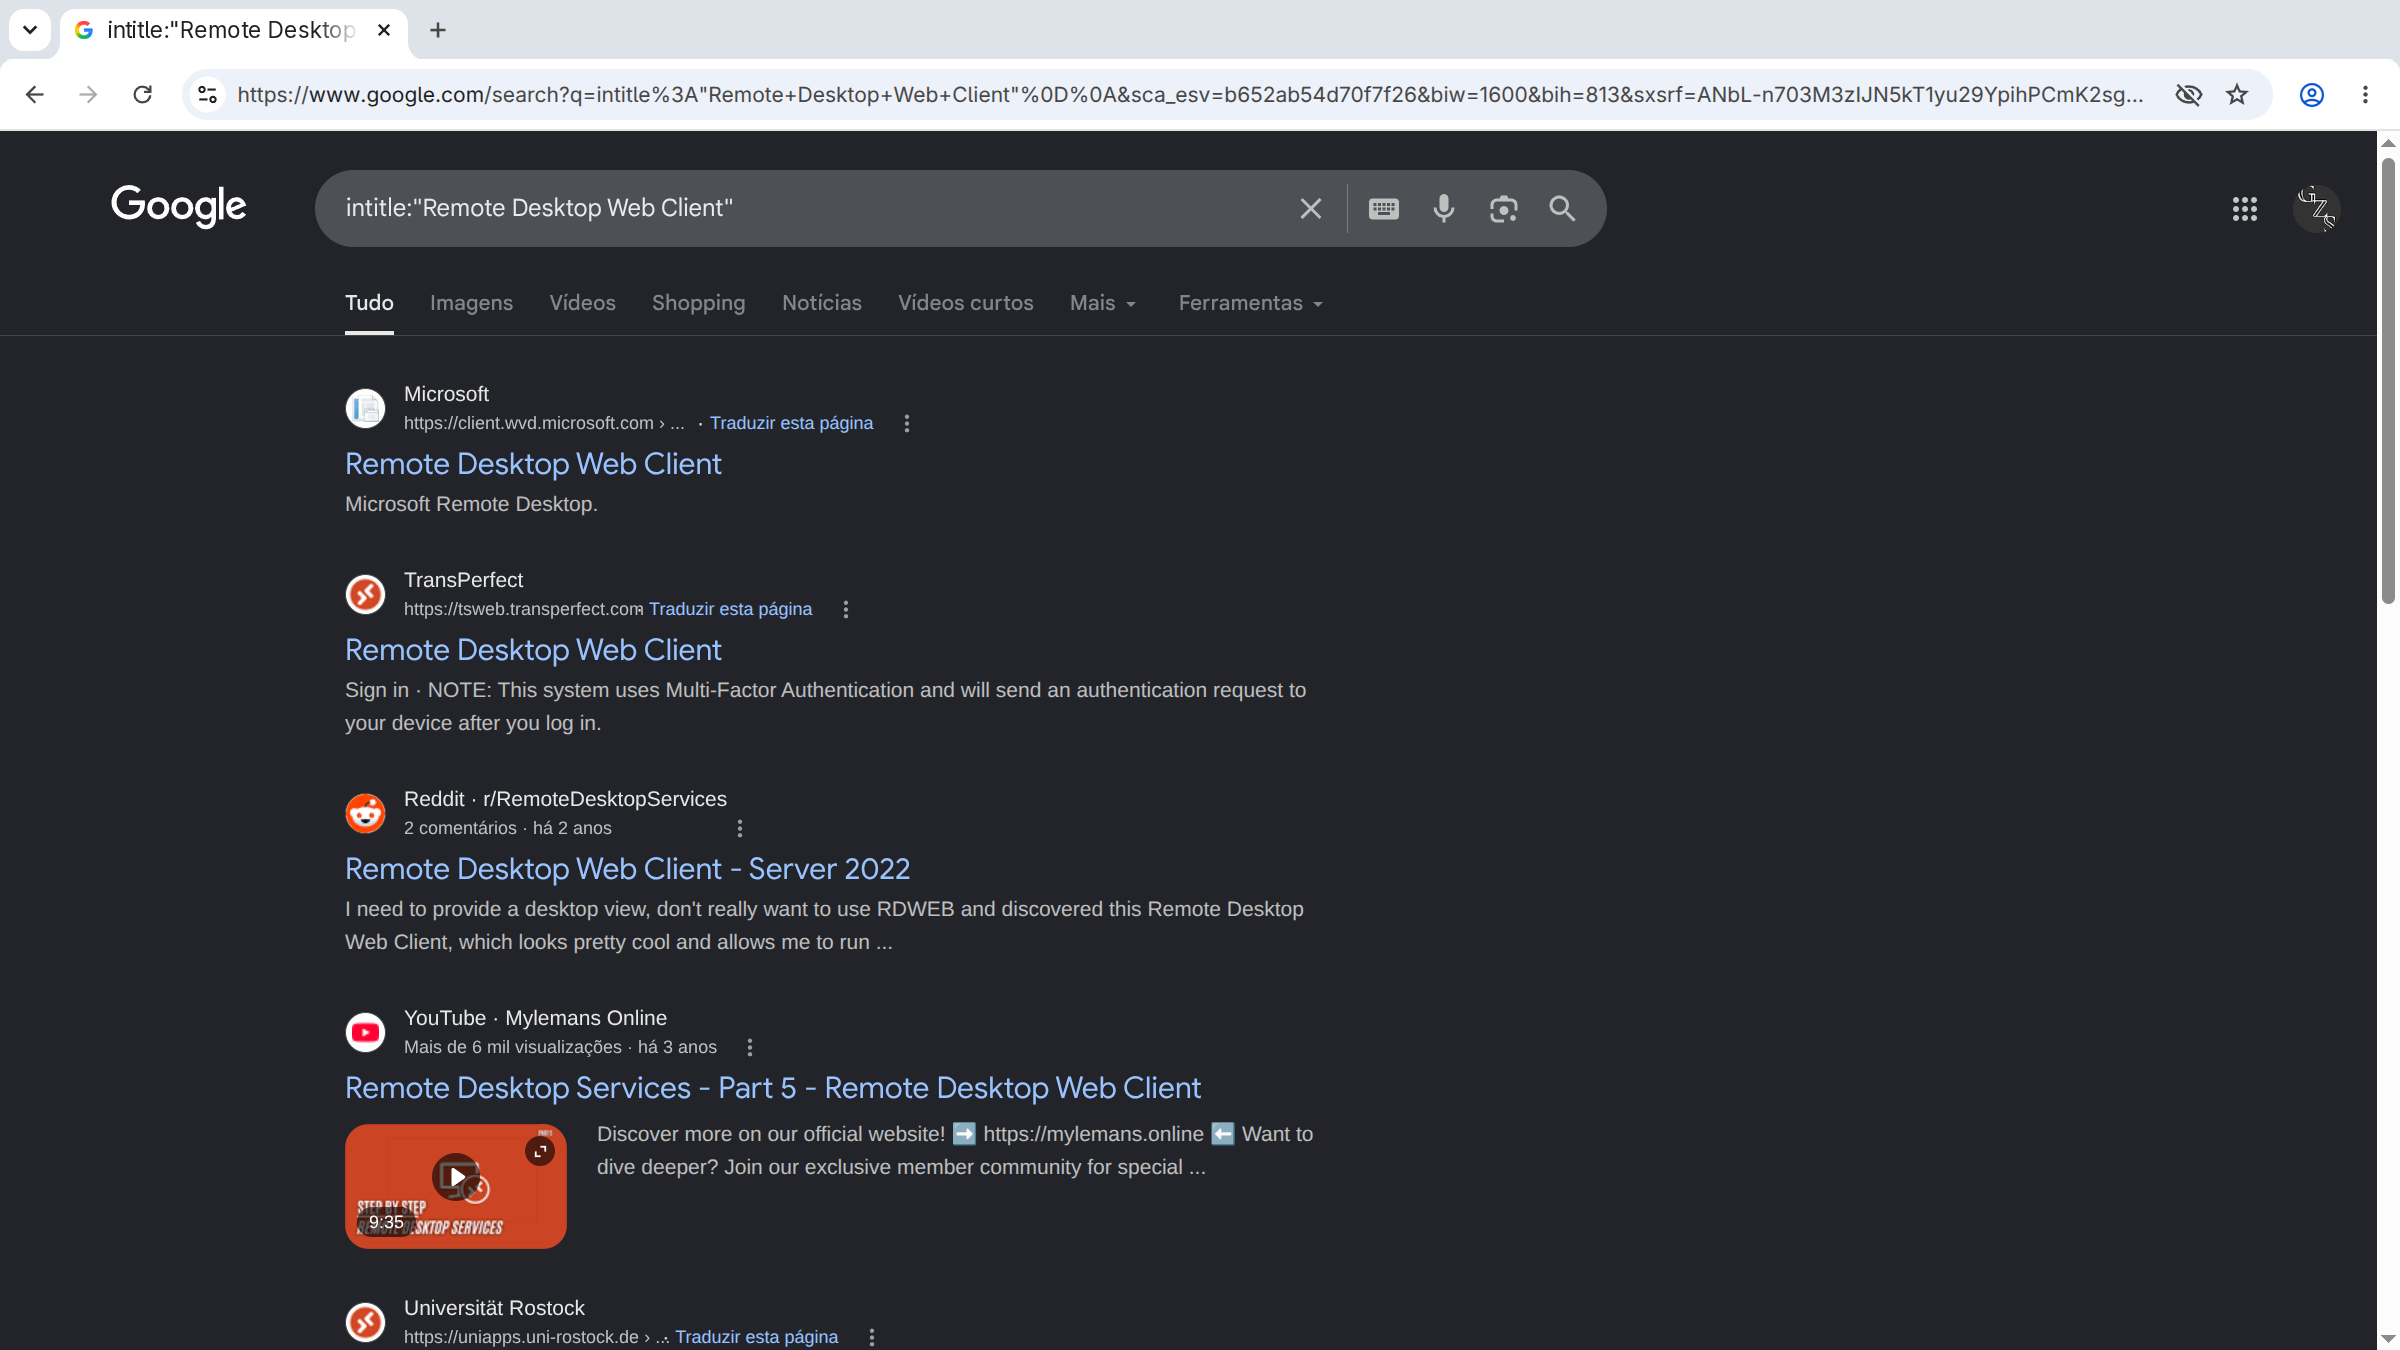
\includegraphics[width=0.95\textwidth]{./fig/atividade5-dork.png}
    \caption{Resultado da pesquisa utilizando Google Dorks.}
\end{figure}

\paragraph{}
Os resultados demonstram como operadores avançados de busca podem ser
utilizados para localizar recursos potencialmente expostos na Internet.
